\documentclass[11pt]{article}
\usepackage[utf8]{inputenc}
% \usepackage[margin=1.5in]{geometry}
\newlength{\alphabet}
\settowidth{\alphabet}{\normalfont abcdefghijklmnopqrstuvwxyz}
\usepackage[textwidth=2.3\alphabet]{geometry}
\usepackage[english]{babel}
\usepackage[dvipsnames]{xcolor}

% --- Paragraphs ---
\usepackage[parfill]{parskip}

% --- Figures ---
\usepackage{float}
\floatplacement{figure}{htb!} % (h)ere (t)op (b)ottom (p)age
\floatplacement{table}{htb!} % (h)ere (t)op (b)ottom (p)age
\usepackage{graphicx}
\graphicspath{{figures/}}
% \usepackage{subcaption}
\usepackage[hidelinks]{hyperref}
% \hypersetup{
%     colorlinks,
%     linkcolor={red!50!black},
%     citecolor={blue!50!black},
%     urlcolor={blue!80!black}
% }


% --- Math ---
\usepackage{amsmath}
\setcounter{MaxMatrixCols}{20}
% \usepackage{nicefrac}

% --- Tables ---
\usepackage{booktabs}
\usepackage{csvsimple}

% --- Fonts ---
\usepackage[babel=true, protrusion=true, expansion=true]{microtype}
\usepackage[T1]{fontenc}
\usepackage{csquotes}
\usepackage[bitstream-charter]{mathdesign}

% \usepackage[format=plain, labelfont=it, textfont=it]{caption}
%% Modify caption labels
\usepackage{caption}
\DeclareCaptionLabelFormat{lc}{\flatcaps{#1}~{#2}}
\captionsetup{font=small, format=plain, labelformat=lc}
% \captionsetup[subfigure]{labelsep=colon, labelfont=sc, labelformat=simple}

%% Lists
\usepackage{enumitem}
\setlist{noitemsep}
\setlist{nosep}
\setlist[1]{labelindent=\parindent} % < Usually a good idea
%% Have to remove the bold and indent labels at the edge, text will still be
%% aligned at \parindent
\setlist[description]{font=\normalfont\flatcaps, labelindent=0pt}

% --- Section Headings ---
%% "Proper" small caps
\newcommand{\flatcaps}[1]{\textsc{\MakeLowercase{#1}}}
%% 'compact' reduces the space above and below headings to a single blank line
\usepackage[compact]{titlesec}
\titleformat{\section}{\large\bfseries}{\thesection}{1em}{}
%% Upright (normal) numbers here
\titleformat{\subsection}{\large}{\thesubsection}{.6em}{\flatcaps}
%% Below, both heading should form sentences
\titleformat{\subsubsection}{}{\thesubsubsection}{.6em}{}{\itshape}
% \titleformat{\paragraph}[runin]{\flatcaps}{\theparagraph}{0pt}{}
\titlespacing*{\section}{0pt}{2\baselineskip}{1\baselineskip}
\titlespacing*{\subsection}{0pt}{1\baselineskip}{1\baselineskip}
\titlespacing*{\subsubsection}{0pt}{8pt}{5pt}


% --- Citations ---
\usepackage[style=apa,sortcites=true,sorting=nyt,backend=biber]{biblatex}
% TODO Following does not seem to work in subdirectory where it should be!
\addbibresource{ref.bib}

% --- Header --- 

\title{A Careful Consideration of the St.\,Petersburg Paradox}
\author{Alexander R. Koen}
\date{\today}

\begin{document}
\maketitle
% \frenchspacing
\tableofcontents

\section{The Paradox}

The St.\,Petersburg paradox is a famous problem in decision theory about a simple game, played as follows:

\begin{enumerate}
\item A coin is flipped repeatedly until, on turn $n$, it lands on heads.
\item The player is awarded $\$2^n$.
\end{enumerate}


  Therefore, as shown in Figure~\ref{fig:distribution}, the game's possible winnings are geometrically distributed with $Pr(\$2^n)=\frac{1}{2}^{n}$. For example, the player has a 50\% chance of winning \$2, a one-quarter chance of winning \$4, a one-eighth chance of winning \$8, and so on.

The paradox is that the expected value of the game is \textit{infinite}, yet no reasonable person would pay more than a few dollars to play.

\begin{figure}
  \centering
  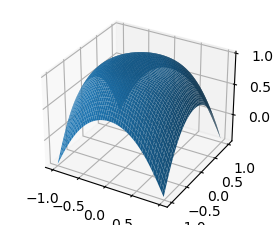
\includegraphics[width=\textwidth]{distribution}
  \caption{Distribution of payouts in one round of the St.\,Petersburg game.}
  \label{fig:distribution}
\end{figure}


\begin{align}
\label{eq:1}
  EMV &= \sum_{n=1}^{\infty} \frac{1}{2^{n}}2^n \\
      &= \sum_{n=1}^{\infty}1 \\
      &= \infty
\end{align}

On the surface, the answer is simple. It's irrational to pay a lot to play because the odds of winning a large sum are extremely low. In other words, because the distribution of possible winnings is long-tailed---that is to say highly non-Gaussian---the mean is a poor measure of central tendency. To illustrate, Table~\ref{tab:world} and Figure~\ref{fig:world} show the distribution of payouts when one round of the game is simulated for $n=7,900,900$ or approximately the global population. While half a dozen people win a \textit{billion dollars} or more, the overwhelming majority take home only small change.

Clearly, expected utility maximization---a core tenet of classical decision theory---fails for this game. However, if the rational price to pay is \textit{not} infinite, then what is it?

\begin{table}
  \centering
  \begin{tabular}{cc}
    \toprule
    \textbf{Winnings (\$)} & \textbf{Number of People} \\
    \midrule
    1 & 5022 \\
2 & 2521 \\
3 & 1255 \\
4 & 609 \\
5 & 314 \\
6 & 142 \\
7 & 68 \\
8 & 34 \\
9 & 15 \\
10 & 11 \\
11 & 5 \\
12 & 3 \\
13 & 1 \\
14 & 0 \\
15 & 0 \\
16 & 0 \\
17 & 0 \\
    \bottomrule
  \end{tabular}
  \caption{Simulated St.\,Petersburg game payouts for $n=7,900,000,000$.}
  \label{tab:world}
\end{table}

\begin{figure}
  \centering
  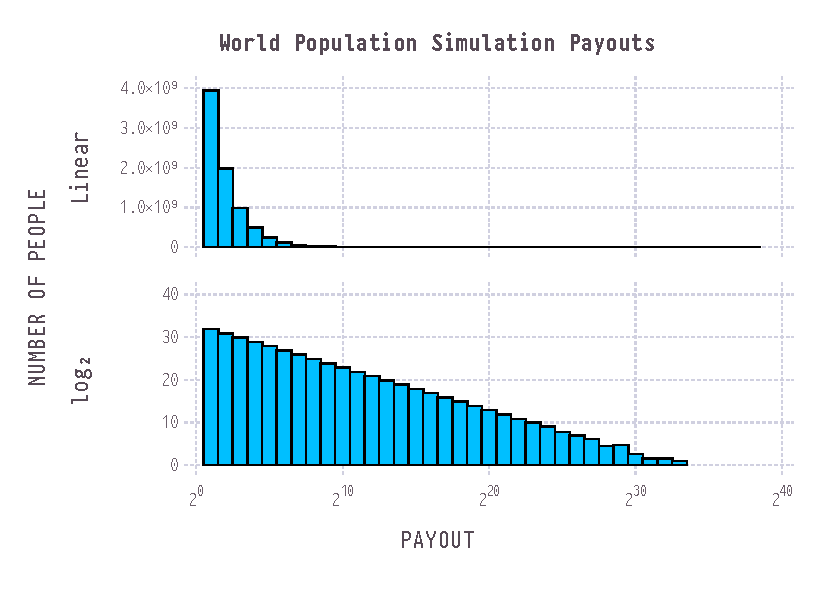
\includegraphics[width=\textwidth]{world}
  \caption{Distribution of simulated St.\,Petersburg game payouts for $n=7,900,000,000$.}
  \label{fig:world}
\end{figure}


% \clearpage
\section{Historical Solutions}
\subsection{Finite funds}
In 1754, Alexis Fontaine presented the paradox to the French \textit{Académie royale des sciences} \parencite[429]{des1764memoires}. He made the case that since the house cannot possibly have infinite funds the expected value may be calculated. For example, if the house has a bankroll of~\$$1,000,000$:
\nopagebreak
\begin{align*}
  \text{Rounds}_{\text{max}} &= \log_2{1000,000,000} \\
                             &\approx 30 \\
                          EU &= \sum_{n=1}^{30}1 \\
                             &\approx 30
\end{align*}


This solution is sensible albeit dissatisfying. Sure, no real-life house can offer an infinite reward. However, the paradox is that even \textif{if they were}, no one would be willing to pay the expected value to play.

\subsection{Expected Utility}
A classic resolution, introduced by \textcite{risk1954exposition}, makes the important observation that in general, EU $\ne$ EMV. He proposed a logarithmic utility function where $U=\ln(\mathrm{MV})$. Consequently, the paradox can be reformulated as follows:

\begin{align*}
  EU &= \sum_{n=1}^{\infty}\left(\frac{1}{2}\right)^n\ln\left(2^n\right) \\
     &= 2\ln 2 \\
\end{align*}
Thus one should be willing to pay $e^{2\ln 2}=\$4$ to play. Others have extended this idea to consider the player's existing wealth~\parencite{petersTimeResolutionSt2011}. 
\[
  \Delta EU=\sum_{n=1}^{\infty}\left(\frac{1}{2}\right)^{n}\left[\overbrace{\ln \left(w-c+2^{n-1}\right)}^{\text {utility after the game }}-\underbrace{\ln (w)}_{\text {utility before the game }}\right],
\]
where $w$ is the player's wealth and $c$ is the cost of a round of play.

These solutions and other variations are again sensible. However, they all may be defeated by increasing the payouts. For example, if the utility function is defined to be $U=\ln(\mathrm{MV})$, then the payouts are simply increased to \$$e^{2n}$:

\begin{align*}
  EU &= \sum_{n=1}^{\infty}\left(\frac{1}{2}\right)^n\ln\left(e^{2n}\right) \\
     &= \infty \\
\end{align*}


\section{Towards a Better Solution}

One may wonder whether a better strategy may be divised when multiple rounds of the game are played. Clearly, in this scenario a rational player should be willing to pay more per round as they have more chance to get lucky.

Figure~\ref{fig:average-over-time} plots the average payout per round against the number of rounds played for 5 random simulations. It is interesting to note that while the results vary greatly, in general they seem to follow a linear trendline.

\begin{figure}
  \centering
  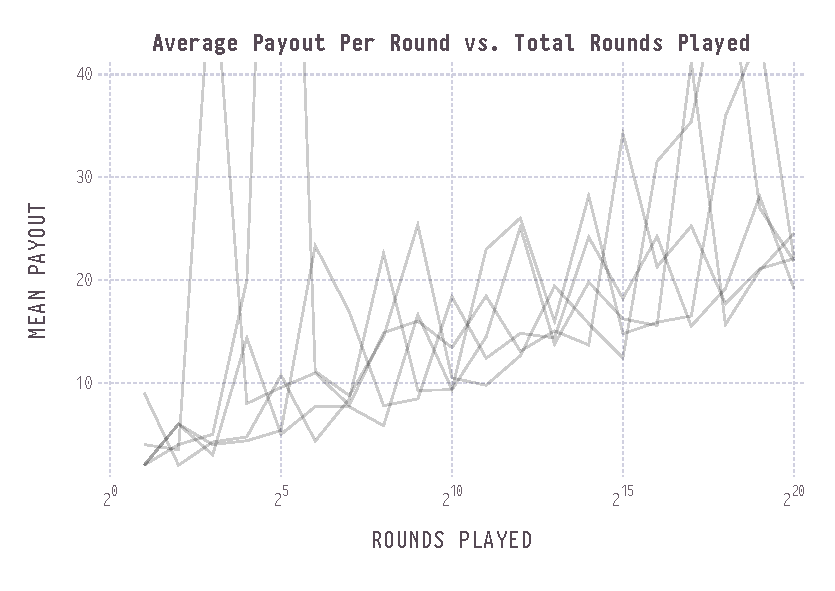
\includegraphics[width=\textwidth]{average-over-time}
  \caption{Mean payout of St.\,Petersburg game after $n$ rounds for five random simulations.}
  \label{fig:average-over-time}
\end{figure}

\clearpage
\subsection{The Steinhaus Sequence}
\begin{minipage}{\textwidth}
To understand why, it is necessary to restate the problem. To do so, consider an empty sequence of infinite length. Now fill every \textit{other} empty space with a 2\dots

\[\begin{bmatrix}{\color{RawSienna} 2} & \_ & {\color{RawSienna} 2} & \_ & {\color{RawSienna} 2} & \_ & {\color{RawSienna} 2} & \_ & {\color{RawSienna} 2} & \_ & {\color{RawSienna} 2} & \_ & {\color{RawSienna} 2}\dots\end{bmatrix} \]

Again, fill every other empty space with a 4\dots

\[\begin{bmatrix}2 & {\color{RawSienna} 4} & 2 & \_ & 2 & {\color{RawSienna} 4} & 2 & \_ & 2 & {\color{RawSienna} 4} & 2 & \_ & 2\dots\end{bmatrix} \]

Once more, now with 8s\dots

\[\begin{bmatrix}2 & 4 & 2 & {\color{RawSienna} 8} & 2 & 4 & 2 & \_ & 2 & 4 & 2 & {\color{RawSienna} 8} & 2\dots\end{bmatrix} \]

And so on\dots\\\\
\end{minipage}
This approach was first proposed by~\textcite{Steinhaus1949}, whose sequence represents exactly the expected payouts of the St.\,Petersburg game. A random draw from elements in the sequence will produce a 2 half the time, a 4 one-quarter of the time, an 8 one-eighth of the time, and so forth. What's more, values are spaced as they are likely to appear at random. While two large values could in theory appear adjacent to one another, entropy favours an even distribution.

Now, the important observation to make is that if this sequence represents expected payouts of the game then it should also represent a fair price to play. For example, if a rational agent has the opportunity to play 3 rounds then he should be willing to pay \$2+\$4+\$2=\$8, or \$2.70 per round to play.

Table~\ref{tab:fair} records these values for numbers of rounds equal to powers of two. At 4 rounds, the fair price is \$4. At 8 rounds, it's \$5. At 16, \$6. Clearly, at pattern has emerged---the fair price is given by \$$log_2n+2$, where $n$ is the number of rounds played. This result is verified by Figure~\ref{fig:steinhaus}. While the cumulative average is less than this value when $n$ is not a power of 2, it is always within \$1.

\begin{table}
  \centering
  \begin{tabular}{ccc}
    \toprule
    \textbf{Number of Rounds} & \textbf{Fair Price [\$]} & \textbf{Fair Price Per Round [\$]} \\
    \midrule
    4  & 16  & 4 \\
    8  & 40  & 5 \\
    16 & 96  & 6 \\
    32 & 224 & 7 \\
    \bottomrule
  \end{tabular}
  \caption{Fair per-round prices for the St.\,Petersburg game.}
  \label{tab:fair}
\end{table}

\begin{figure}
  \centering
  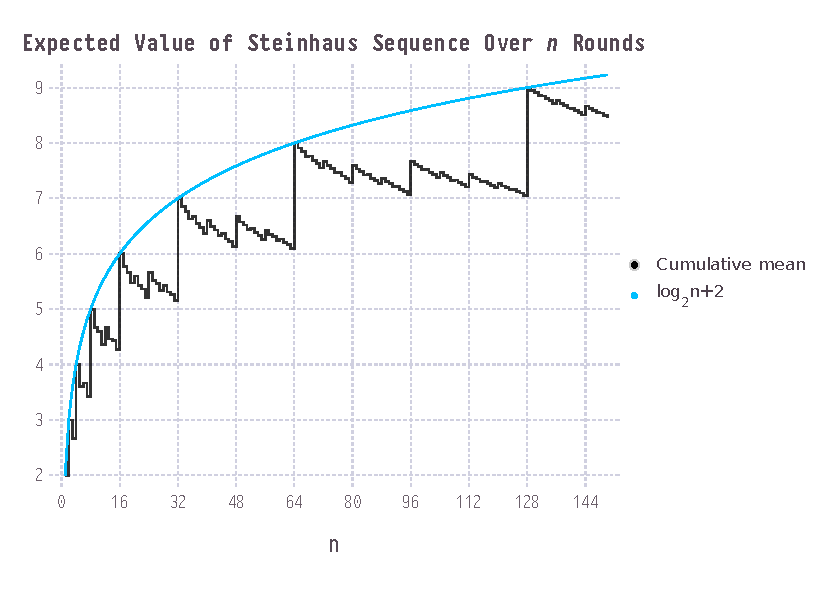
\includegraphics[width=\textwidth]{steinhaus}
  \caption{Cumulative averages of the Steinhaus sequence plotted against $log_2n+2$.}
  \label{fig:steinhaus}
\end{figure}

Naturally, these findings should be tested experimentally. Figure~\ref{fig:average-over-time-fit} overlays the simulated mean payouts over $n$ rounds from Figure~\ref{fig:average-over-time} with the fair price \$$log_2n+2$. It is remarkably accurate.

\begin{figure}
  \centering
  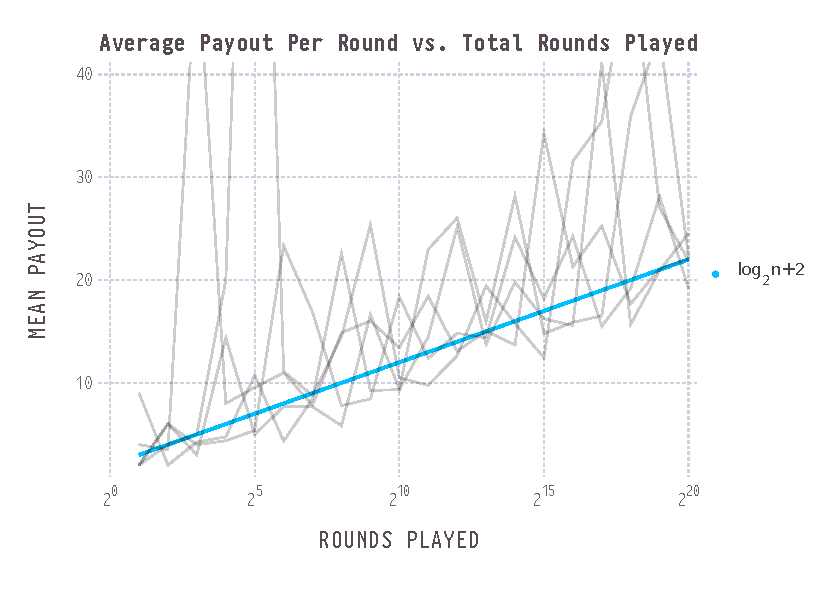
\includegraphics[width=\textwidth]{average-over-time-fit}
  \caption{Average payout after $n$ games, plotted against \$$\log_2n+2$.}
  \label{fig:average-over-time-fit}
\end{figure}

\clearpage
\section{Simulations}

The following simulations presented in Figure~\ref{fig:evolution} plot the wealth of 1,000 players over 10,000 rounds of the game with per-round fees of (a) \$2 and (b) \$100. 

\begin{figure}
  \centering
  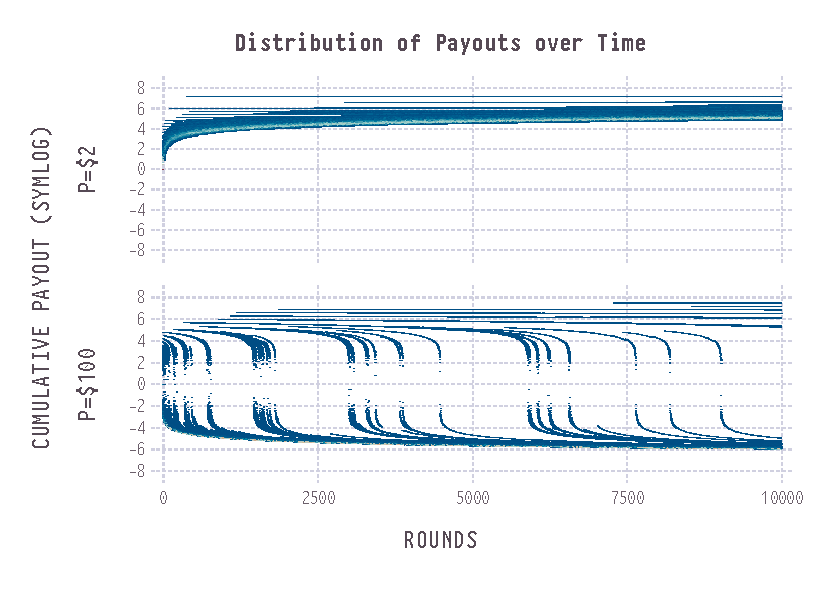
\includegraphics[width=\textwidth]{winnings-2-100}
  \caption{Evolution of cumulative payout for 1,000 simulated players over 10,000 rounds of the St.\,Petersburg game with per-round fees of \$2 and \$100. Y-axis plotted on a \textit{symmetrical log (symlog)} scale $\left(Y=\mathrm{sgn}(y)\log_{10}|y+1|\right)$.}
  \label{fig:evolution}
\end{figure}

Clearly, \$2 is too low while \$100 is too high. However, it is interesting to note the asymmetry in their evolution. At \$2, players' wealth always increases. At \$100, however, only the very lucky---represented by horizontal lines on the positive y-axis---can weather the attraction towards debt. However, at the limit, they too will suffer the inevitable s-shaped fall from grace.

By contrast, Figure~\ref{fig:evolution-fair} plots the same simulations with a per-round fee set to $\$log_210,000+2$ or $\approx\$15$. While players lose money on most rounds, this is offset by the occasional large payout. Consequently, wealth is asymptotically stable---the game is fair.

\begin{figure}
  \centering
  \includegraphics[width=\textwidth]{winnings-N}
  \caption{Evolution of cumulative payout for 1,000 simulated players over 10,000 rounds of the St.\,Petersburg game with a per-round fee of $log_2(10,000)+2\approx\$15$. At this price wealth is asymptotically stable. Y-axis plotted on symmetrical log (symlog) scale. Zoom in.} \label{fig:evolution-fair}
\end{figure}

\clearpage
\section{Conclusion}

As with any game of chance, there will never be a completely ``correct'' solution to the St.\,Petersburg Paradox. Strategy will always depend on an individual player's risk tolerance, wealth, and other factors. However, the strategy presented in this paper---that a rational person should be willing to pay $\$log_2n+2$ per-round---is convincing. While the intersection of people with an interest in logical paradoxes and those will unlimited finances may be too limited to test these strategies in the real world, it is at least a fascinating idea to explore.


Source code for all figures and simulations is available at \url{https://github.com/akoen/petersburg}. Made using Julia and Gadfly \footcite{daniel_c_jones_2021_5559613}.
\clearpage
\printbibliography
\end{document}

% Local Variables:
% TeX-engine: luatex
% End:
